\documentclass[border=10pt]{standalone}

\usepackage{verbatim}


% my addons
\usepackage{graphicx}

%img path
\graphicspath{ {/home/propeller/Downloads/} }
%end of my addons


\usepackage[utf8]{inputenc}
\usepackage{tikz}
\usetikzlibrary{arrows.meta}
\usetikzlibrary{mindmap,shadows}
\usepackage[hidelinks,pdfencoding=auto]{hyperref}

% Information boxes
\newcommand*{\info}[4][16.3]{%
  \node [ annotation, #3, scale=0.65, text width = #1em,
          inner sep = 2mm ] at (#2) {%
  \list{$\bullet$}{\topsep=0pt\itemsep=0pt\parsep=0pt
    \parskip=0pt\labelwidth=8pt\leftmargin=8pt
    \itemindent=0pt\labelsep=2pt}%
    #4
  \endlist
  };
}


%Extra color defined 
\definecolor{tempGrn}{RGB}{221, 221, 187}
\definecolor{tempBlock}{RGB}{242,204,255}
\definecolor{tempSec}{RGB}{212,170,19}
\definecolor{tempCom}{RGB}{179, 236, 255}
\definecolor{tempE}{RGB}{179, 209, 255}
\definecolor{tempD}{RGB}{153, 153, 255}
%end of extra color

\begin{document}
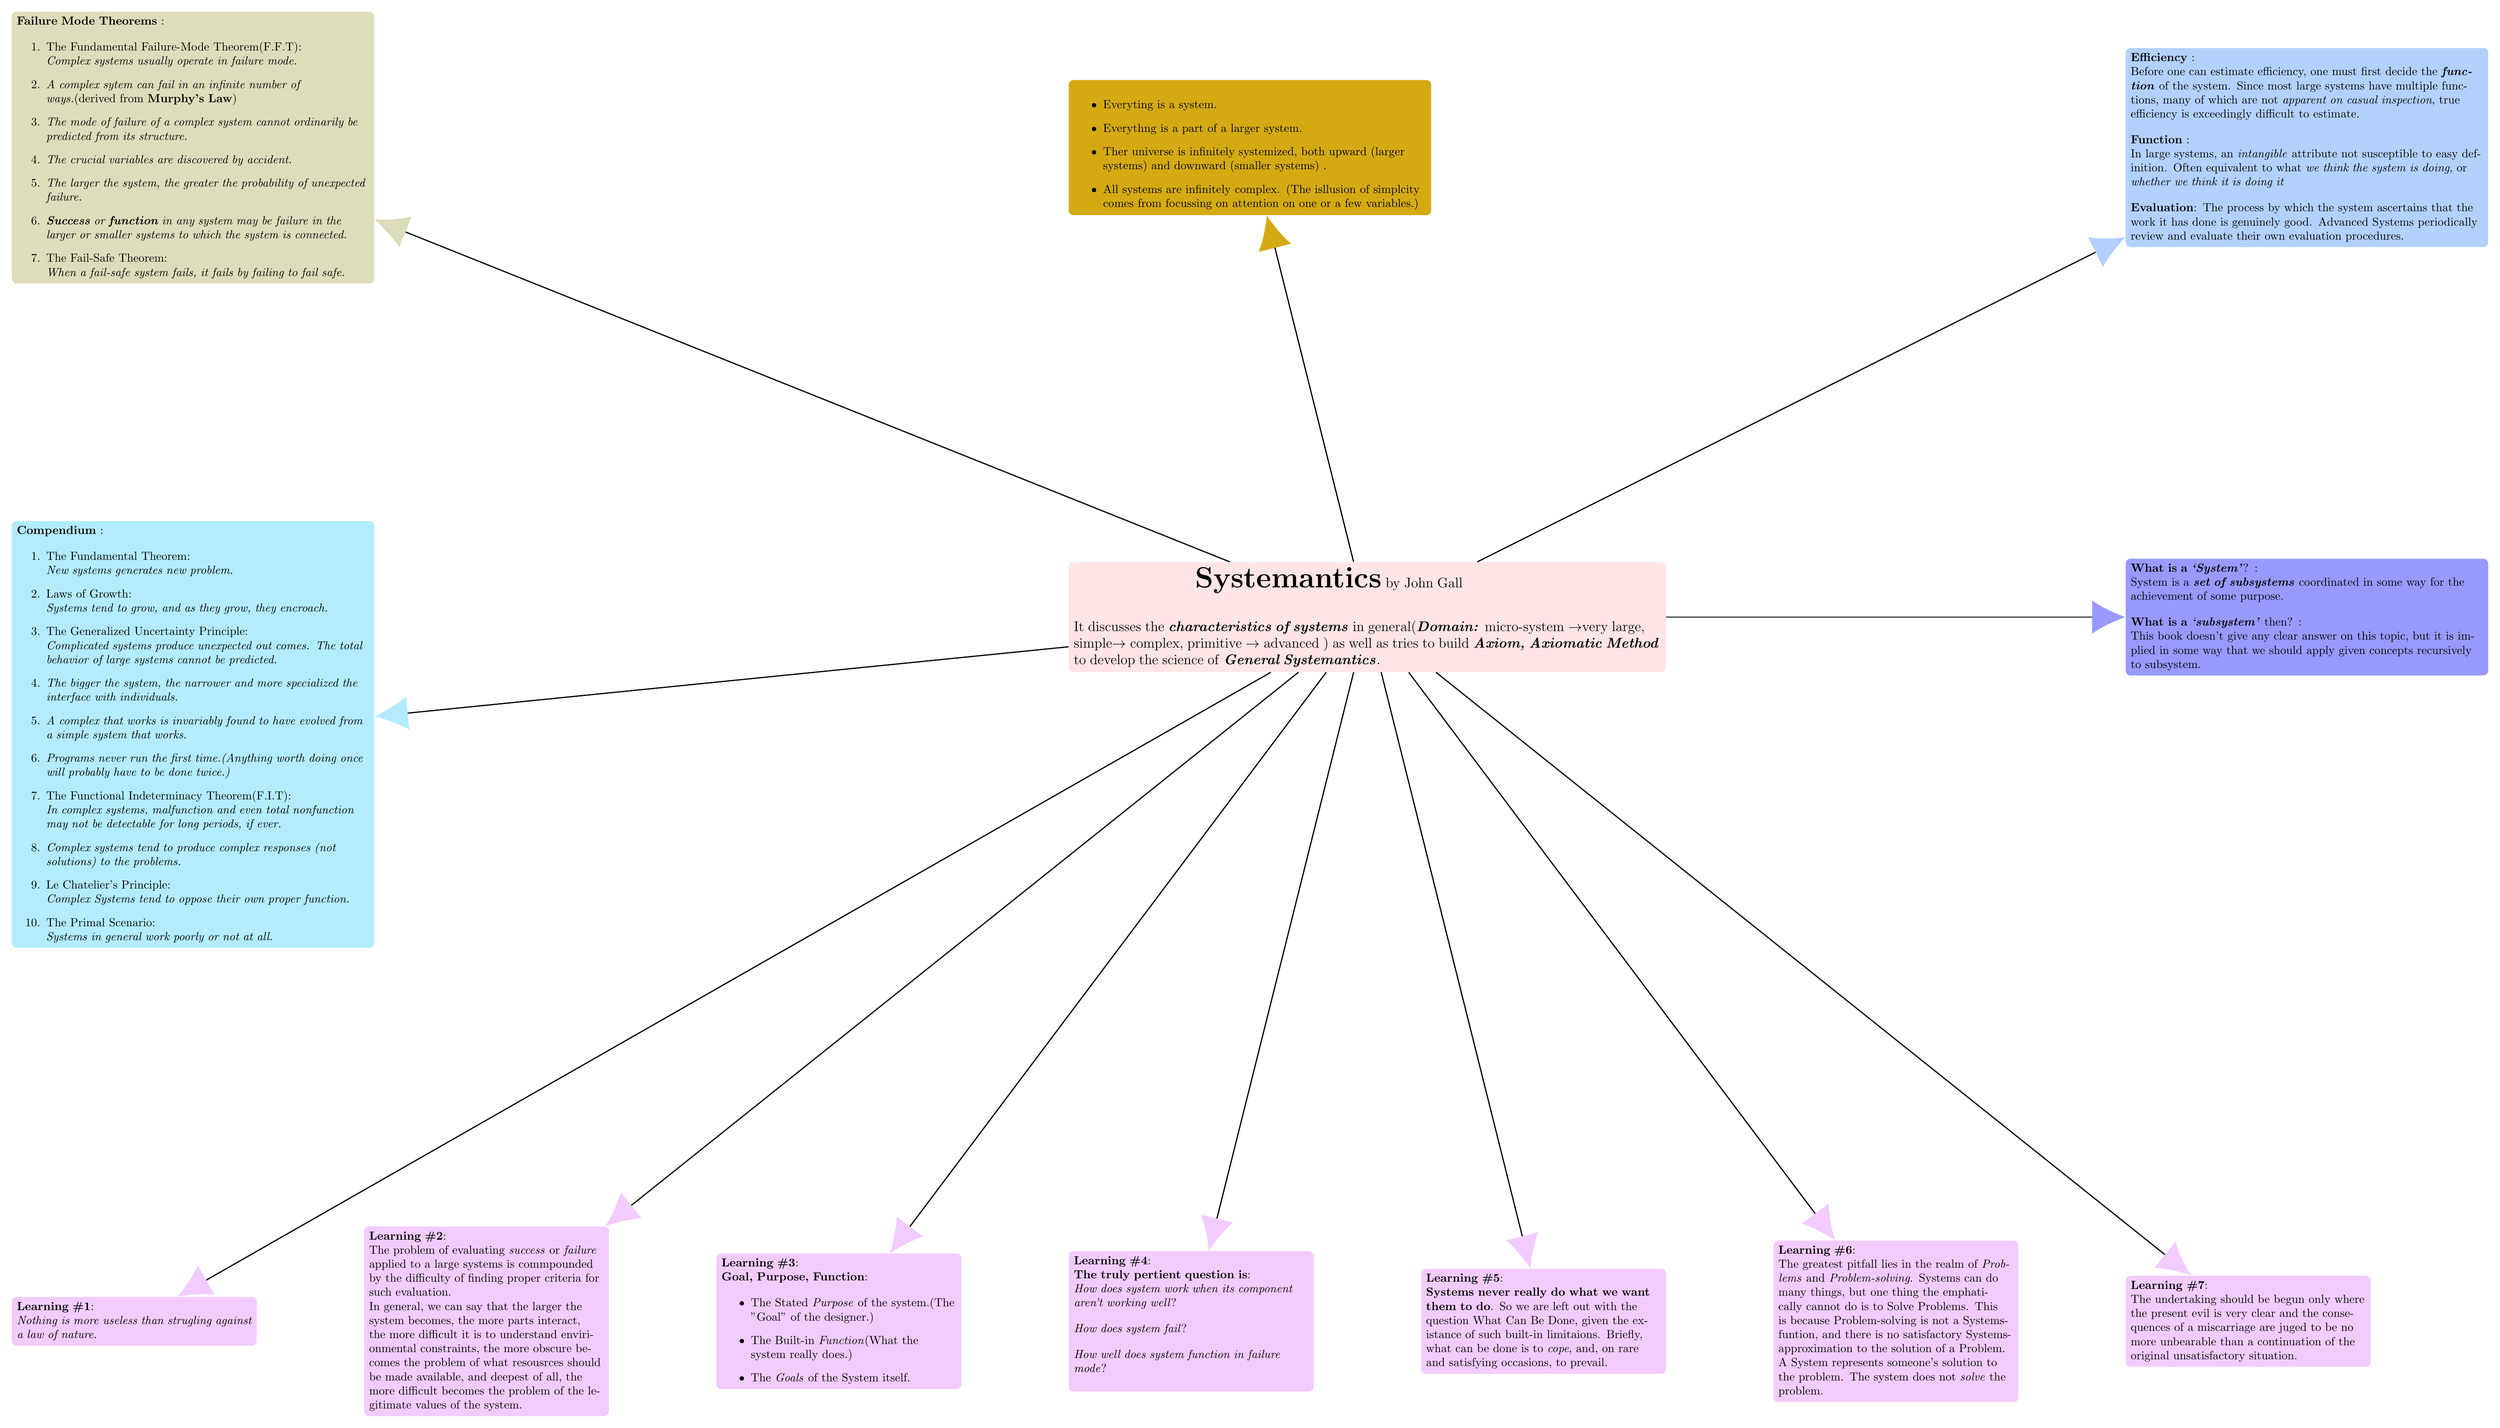
\begin{tikzpicture}
[
% Styles
information text/.style={rounded corners,fill=red!10,inner sep=1ex}]
information/.style={rounded corners,fill=red!10,inner sep=1ex}]
% Local definitions

\draw[xshift=30em,yshift=10em]
node[right,text width=50em,information text](first)
{
\hspace{10em} \Huge{\textbf{Systemantics}} \large  by John Gall\\
\vspace{2em}
It discusses the \textbf{\textit{characteristics of systems}} in general(\textbf{\textit{Domain:}} micro-system $\rightarrow $very large, simple$\rightarrow$ complex, primitive $\rightarrow$ advanced ) as well as tries to build \textbf{\textit{Axiom, Axiomatic Method}} to develop the science of \textbf{\textit{General Systemantics}}.
 
};
\draw[yshift=50em, xshift=30em]
node[right,text width=30em,information text,fill=tempSec](second)
{
\begin{itemize}
\item Everyting is a system.
\item Everythng is a part of a larger system.
\item Ther universe is infinitely systemized, both upward (larger systems) and downward (smaller systems) .
\item All systems are infinitely complex. (The isllusion of simplcity comes from focussing on attention on one or a few variables.)
\end{itemize}
};


\draw[yshift=10em, xshift=120em]
node[right,text width=30em,information text,fill=tempD](def)
{
\textbf{What is a \textit{`System'}}? :\\
System is a \textbf{\textit{set of subsystems}} coordinated in some way for the achievement of some purpose.\\
\vspace{1em}
\textbf{What is a \textit{`subsystem'}} then? :\\
This book doesn't give any clear answer on this topic, but it is implied in some way that we should apply given concepts recursively to subsystem.
};


%..........................................
\draw[yshift=50em, xshift=120em]
node[right,text width=30em,information text,fill=tempE](tempE)
{
\textbf{Efficiency} :\\
Before one can estimate efficiency, one must first decide the \textbf{\textit{function}} of the system. Since most large systems have multiple functions, many of which are not \textit{apparent on casual inspection}, true efficiency is exceedingly difficult to estimate.\\
\vspace{1em}
\textbf{Function} :\\
In large systems, an \textit{intangible} attribute not susceptible to easy definition. Often equivalent to what \textit{we think the system is doing}, or \textit{whether we think it is doing it}\\
\vspace{1em}
\textbf{Evaluation}:
The process by which the system ascertains that the work it has done is genuinely good. Advanced Systems periodically review and evaluate their own evaluation procedures.
};
%.............................................


%.............................................
\draw[ xshift=-60em]
node[right,text width=30em,information text,fill=tempCom](com)
{
\textbf{Compendium} :\\
\begin{itemize}
\item[1.] The Fundamental Theorem:\\
\textit{New systems generates new problem.}
\item[2.] Laws of Growth:\\
\textit{Systems tend to grow, and as they grow, they encroach.}
\item[3.] The Generalized Uncertainty Principle:\\
\textit{Complicated systems produce unexpected out comes. The total behavior of large systems cannot be predicted.}
\item[4.]\textit{The bigger the system, the narrower and more specialized the interface with individuals.}
\item[5.]\textit{A complex that works is invariably found to have evolved from a simple system that works.}
\item[6.]\textit{Programs never run the first time.(Anything worth doing once will probably have to be done twice.)}
\item[7.] The Functional Indeterminacy Theorem(F.I.T):\\
\textit{In complex systems, malfunction and even total nonfunction may not be detectable for long periods, if ever.}
\item[8.] \textit{Complex systems tend to produce complex responses (not solutions) to the problems.}
\item[9.]Le Chatelier's Principle:\\
\textit{Complex Systems tend to oppose their own proper function.}
\item[10.] The Primal Scenario:\\
\textit{Systems in general work poorly or not at all.}

\end{itemize}
};


%............................
\draw[yshift=50em, xshift=-60em]
node[right,text width=30em,information text,fill=tempGrn](fMode)
{
\textbf{Failure Mode Theorems} :\\
\begin{itemize}
\item[1.] The Fundamental Failure-Mode Theorem(F.F.T):\\
\textit{Complex systems usually operate in failure mode.}
\item[2.] \textit{A complex sytem can fail in an infinite number of ways.}(derived from \textbf{Murphy's Law})
\item[3.] \textit{The mode of failure of a complex system cannot ordinarily be predicted from its structure.}
\item[4.]\textit{The crucial variables are discovered by accident.}
\item[5.]\textit{The larger the system, the greater the probability of unexpected failure.}
\item[6.]\textit{\textbf{Success} or \textbf{function} in any system may be failure in the larger or smaller systems to which the system is connected.}
\item[7.]The Fail-Safe Theorem:\\
\textit{When a fail-safe system fails, it fails by failing to fail safe.}

\end{itemize}
};

%............................


%...................................
\draw[yshift=-50em, xshift=-60em]
node[right,text width=20em,information text,fill=tempBlock](1)
{
\textbf{Learning \#1}:\\
\textit{Nothing is more useless than strugling against a law of nature.}
};

\draw[yshift=-50em, xshift=-30em]
node[right,text width=20em,information text,fill=tempBlock](2)
{
\textbf{Learning \#2}:\\
The problem of evaluating \textit{success} or \textit{failure} applied to a large systems is commpounded by the difficulty of finding proper criteria for such evaluation.\\
In general, we can say that the larger the system becomes, the more parts interact, the more difficult it is to understand envirionmental constraints, the more obscure becomes the problem of what resousrces should be made available, and deepest of all, the more difficult becomes the problem of the legitimate values of the system.
};
\draw[yshift=-50em, xshift=0em]
node[right,text width=20em,information text,fill=tempBlock](3)
{
\textbf{Learning \#3}:\\
\textbf{Goal, Purpose, Function}:\\
\begin{itemize}
\item The Stated \textit{Purpose} of the system.(The "Goal" of the designer.)
\item The Built-in \textit{Function}(What the system really does.)
\item The \textit{Goals} of the System itself.
\end{itemize}
};

\draw[yshift=-50em, xshift=30em]
node[right,text width=20em,information text,fill=tempBlock](4)
{
\textbf{Learning \#4}:\\
\textbf{The truly pertient question is}:\\
\textit{How does system work when its component aren't working well}?\\
\vspace{1em}
\textit{How does system fail}?\\
\vspace{1em}
\textit{How well does system function in failure mode}?

\
};


\draw[yshift=-50em, xshift=60em]
node[right,text width=20em,information text,fill=tempBlock](5)
{
\textbf{Learning \#5}:\\
\textbf{Systems never really do what we want them to do}. So we are left out with the question What Can Be Done, given the existance of such built-in limitaions. Briefly, what can be done is to \textit{cope}, and, on rare and satisfying occasions, to prevail.
};

\draw[yshift=-50em, xshift=90em]
node[right,text width=20em,information text,fill=tempBlock](6)
{
\textbf{Learning \#6}:\\
The greatest pitfall lies in the realm of \textit{Problems} and \textit{Problem-solving}. Systems can do many things, but one thing the emphatically cannot do is to Solve Problems. This is because Problem-solving is not a Systems-funtion, and there is no satisfactory Systems-approximation to the solution of a Problem. A System represents someone's solution to the problem. The system does not \textit{solve} the problem.
};

\draw[yshift=-50em, xshift=120em]
node[right,text width=20em,information text,fill=tempBlock](7)
{
\textbf{Learning \#7}:\\
The undertaking should be begun only where the present evil is very clear and the consequences of a miscarriage are juged to be no more unbearable than a continuation of the original unsatisfactory situation.
};
%...................................
%\draw[-{>[scale=5.55,
   %       length=10,
      %    width=5]},line width=5pt] (first)  edge [bend right] (second);
          
%\draw[-{Latex[length=5mm, width=2mm]}](first)  edge [bend left] (second);

\draw[-{Latex[tempSec,length=10mm, width=10mm]},line width=1pt](first)  edge (second);

\draw[-{Latex[tempBlock,length=10mm, width=10mm]},line width=1pt](first)  edge (1);
\draw[-{Latex[tempBlock,length=10mm, width=10mm]},line width=1pt](first)  edge (2);
\draw[-{Latex[tempBlock,length=10mm, width=10mm]},line width=1pt](first)  edge (3);
\draw[-{Latex[tempBlock,length=10mm, width=10mm]},line width=1pt](first)  edge (4);
\draw[-{Latex[tempBlock,length=10mm, width=10mm]},line width=1pt](first)  edge (5);
\draw[-{Latex[tempBlock,length=10mm, width=10mm]},line width=1pt](first)  edge (6);
\draw[-{Latex[tempBlock,length=10mm, width=10mm]},line width=1pt](first)  edge (7);


\draw[-{Latex[tempCom,length=10mm, width=10mm]},line width=1pt](first)  edge (com);

\draw[-{Latex[tempGrn,length=10mm, width=10mm]},line width=1pt](first)  edge (fMode);

\draw[-{Latex[tempE,length=10mm, width=10mm]},line width=1pt](first)  edge (tempE);

\draw[-{Latex[tempD,length=10mm, width=10mm]},line width=1pt](first)  edge (def);
\end{tikzpicture}
\end{document}

